% generated by Plantuml 1.2024.2       
\definecolor{plantucolor0000}{RGB}{0,0,0}
\definecolor{plantucolor0001}{RGB}{241,241,241}
\definecolor{plantucolor0002}{RGB}{24,24,24}
\definecolor{plantucolor0003}{RGB}{235,147,127}
\definecolor{plantucolor0004}{RGB}{200,41,48}
\definecolor{plantucolor0005}{RGB}{132,190,132}
\definecolor{plantucolor0006}{RGB}{3,128,72}
\definecolor{plantucolor0007}{RGB}{180,167,229}
\definecolor{plantucolor0008}{RGB}{173,209,178}
\definecolor{plantucolor0009}{RGB}{242,77,92}
\scalebox{0.6}{
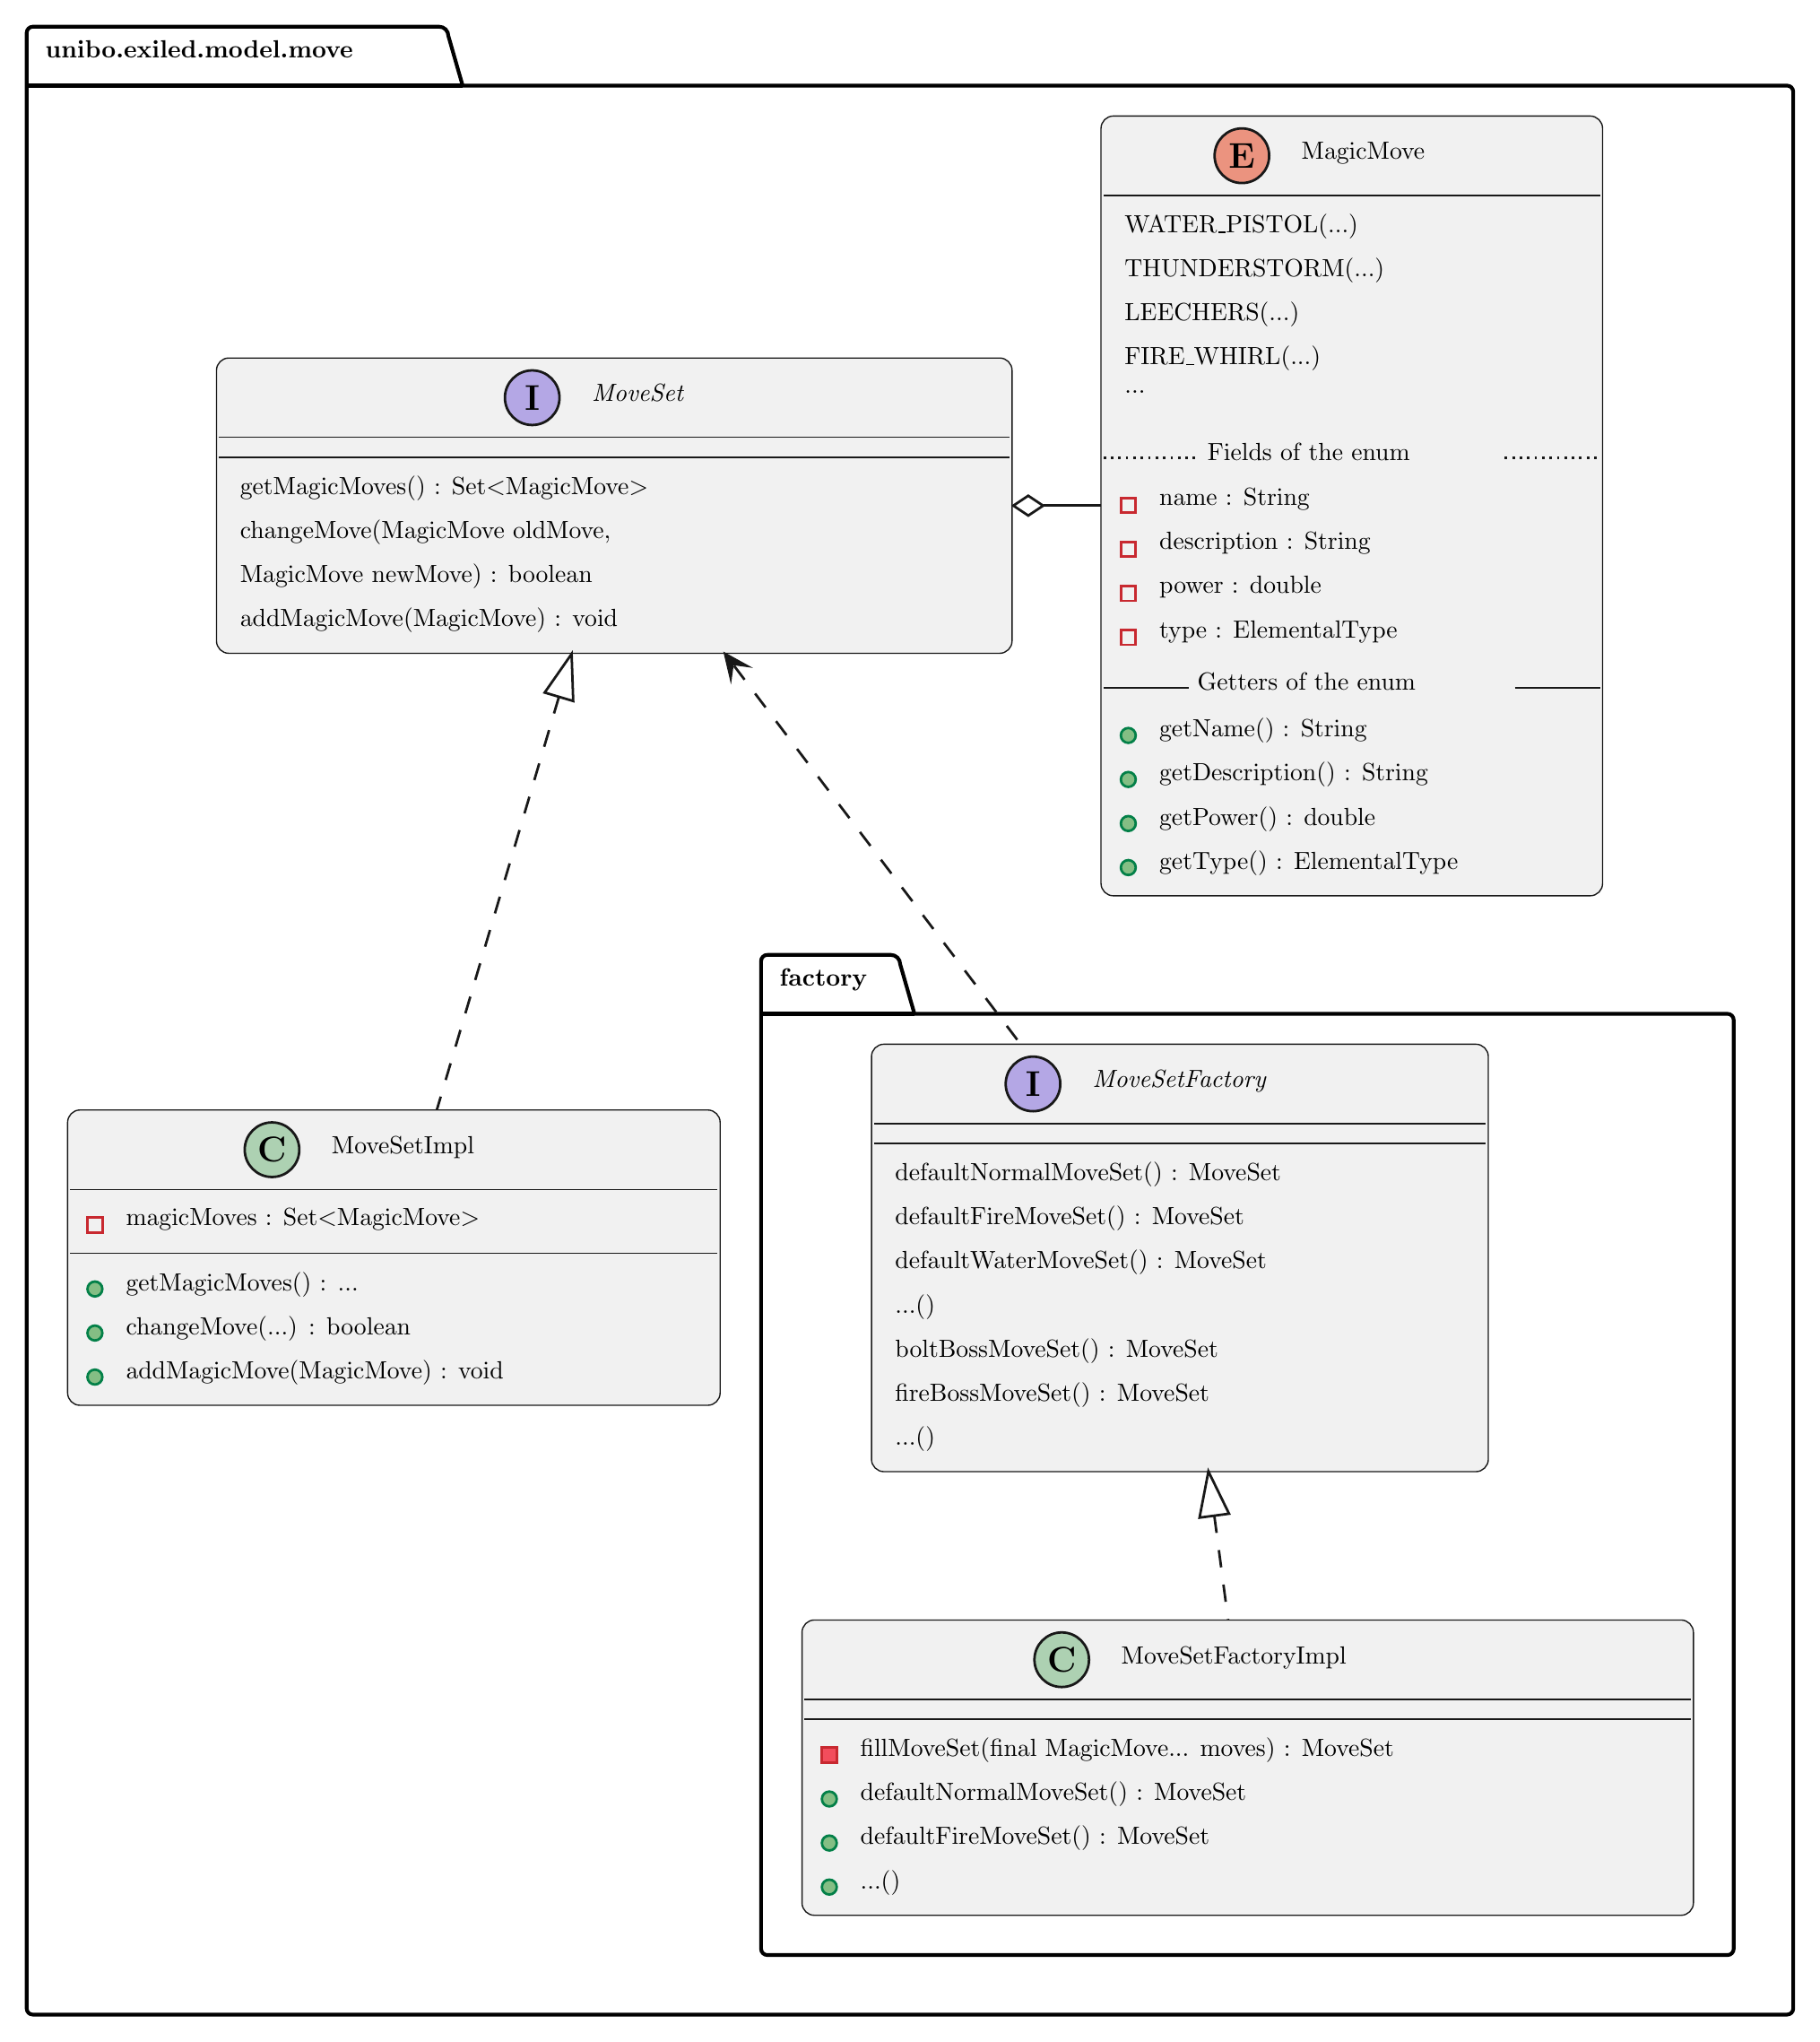
\begin{tikzpicture}[yscale=-1
,pstyle0/.style={color=black,line width=1.5pt}
,pstyle1/.style={color=plantucolor0002,fill=plantucolor0001,line width=0.5pt}
,pstyle3/.style={color=plantucolor0002,line width=0.5pt}
,pstyle4/.style={color=plantucolor0004,line width=1.0pt}
,pstyle5/.style={color=plantucolor0002,line width=1.0pt,dash pattern=on 1.0pt off 2.0pt}
,pstyle6/.style={color=plantucolor0006,fill=plantucolor0005,line width=1.0pt}
,pstyle7/.style={color=plantucolor0002,fill=plantucolor0007,line width=1.0pt}
,pstyle8/.style={color=plantucolor0002,fill=plantucolor0008,line width=1.0pt}
,pstyle10/.style={color=plantucolor0002,line width=1.0pt,dash pattern=on 7.0pt off 7.0pt}
,pstyle11/.style={color=plantucolor0002,line width=1.0pt}
]
\draw[pstyle0] (8.5pt,6pt) -- (172.2158pt,6pt) arc(270:360:3.75pt)  -- (181.7158pt,29.7461pt) -- (715.5pt,29.7461pt) arc(270:360:2.5pt)  -- (718pt,804.5pt) arc(0:90:2.5pt)  -- (8.5pt,807pt) arc(90:180:2.5pt)  -- (6pt,8.5pt) arc(180:270:2.5pt) ;
\draw[pstyle0] (6pt,29.7461pt) -- (181.7158pt,29.7461pt);
\node at (10pt,8pt)[below right,color=black]{\textbf{unibo.exiled.model.move}};
\draw[pstyle0] (304.5pt,380pt) -- (354.3093pt,380pt) arc(270:360:3.75pt)  -- (363.8093pt,403.7461pt) -- (691.5pt,403.7461pt) arc(270:360:2.5pt)  -- (694pt,780.5pt) arc(0:90:2.5pt)  -- (304.5pt,783pt) arc(90:180:2.5pt)  -- (302pt,382.5pt) arc(180:270:2.5pt) ;
\draw[pstyle0] (302pt,403.7461pt) -- (363.8093pt,403.7461pt);
\node at (306pt,382pt)[below right,color=black]{\textbf{factory}};
\draw[pstyle1] (439pt,47pt) arc (180:270:5pt) -- (444pt,42pt) -- (636.16pt,42pt) arc (270:360:5pt) -- (641.16pt,47pt) -- (641.16pt,351.1914pt) arc (0:90:5pt) -- (636.16pt,356.1914pt) -- (444pt,356.1914pt) arc (90:180:5pt) -- (439pt,351.1914pt) -- cycle;
\draw[color=plantucolor0002,fill=plantucolor0003,line width=1.0pt] (495.7793pt,58pt) ellipse (11pt and 11pt);
\node at (495.7793pt,58pt)[]{\textbf{\Large E}};
\node at (516.2793pt,49.127pt)[below right,color=black]{MagicMove};
\draw[pstyle3] (440pt,74pt) -- (640.16pt,74pt);
\node at (445pt,78pt)[below right,color=black]{WATER\_PISTOL(...)};
\node at (445pt,95.7461pt)[below right,color=black]{THUNDERSTORM(...)};
\node at (445pt,113.4922pt)[below right,color=black]{LEECHERS(...)};
\node at (445pt,131.2383pt)[below right,color=black]{FIRE\_WHIRL(...)};
\node at (445pt,148.9844pt)[below right,color=black]{...};
\draw[pstyle4] (447pt,195.8496pt) rectangle (453pt,201.8496pt);
\node at (459pt,188.4766pt)[below right,color=black]{name : String};
\draw[pstyle4] (447pt,213.5957pt) rectangle (453pt,219.5957pt);
\node at (459pt,206.2227pt)[below right,color=black]{description : String};
\draw[pstyle4] (447pt,231.3418pt) rectangle (453pt,237.3418pt);
\node at (459pt,223.9688pt)[below right,color=black]{power : double};
\draw[pstyle4] (447pt,249.0879pt) rectangle (453pt,255.0879pt);
\node at (459pt,241.7148pt)[below right,color=black]{type : ElementalType};
\draw[pstyle5] (440pt,179.6035pt) -- (478.4133pt,179.6035pt);
\node at (478.4133pt,170.2305pt)[below right,color=black]{Fields of the enum};
\draw[pstyle5] (601.7467pt,179.6035pt) -- (640.16pt,179.6035pt);
\draw[pstyle6] (450pt,291.5801pt) ellipse (3pt and 3pt);
\node at (459pt,281.207pt)[below right,color=black]{getName() : String};
\draw[pstyle6] (450pt,309.3262pt) ellipse (3pt and 3pt);
\node at (459pt,298.9531pt)[below right,color=black]{getDescription() : String};
\draw[pstyle6] (450pt,327.0723pt) ellipse (3pt and 3pt);
\node at (459pt,316.6992pt)[below right,color=black]{getPower() : double};
\draw[pstyle6] (450pt,344.8184pt) ellipse (3pt and 3pt);
\node at (459pt,334.4453pt)[below right,color=black]{getType() : ElementalType};
\draw[pstyle3] (440pt,272.334pt) -- (474.3508pt,272.334pt);
\node at (474.3508pt,262.9609pt)[below right,color=black]{Getters of the enum};
\draw[pstyle3] (605.8092pt,272.334pt) -- (640.16pt,272.334pt);
\draw[pstyle1] (82.5pt,144.5pt) arc (180:270:5pt) -- (87.5pt,139.5pt) -- (398.1519pt,139.5pt) arc (270:360:5pt) -- (403.1519pt,144.5pt) -- (403.1519pt,253.4844pt) arc (0:90:5pt) -- (398.1519pt,258.4844pt) -- (87.5pt,258.4844pt) arc (90:180:5pt) -- (82.5pt,253.4844pt) -- cycle;
\draw[pstyle7] (209.7474pt,155.5pt) ellipse (11pt and 11pt);
\node at (209.7474pt,155.5pt)[]{\textbf{\Large I}};
\node at (230.2474pt,146.627pt)[below right,color=black]{\textit{MoveSet}};
\draw[pstyle3] (83.5pt,171.5pt) -- (402.1519pt,171.5pt);
\draw[pstyle3] (83.5pt,179.5pt) -- (402.1519pt,179.5pt);
\node at (88.5pt,183.5pt)[below right,color=black]{getMagicMoves() : Set\textless MagicMove\textgreater };
\node at (88.5pt,201.2461pt)[below right,color=black]{changeMove(MagicMove oldMove,};
\node at (88.5pt,218.9922pt)[below right,color=black]{                     MagicMove newMove) : boolean};
\node at (88.5pt,236.7383pt)[below right,color=black]{addMagicMove(MagicMove) : void};
\draw[pstyle1] (22.5pt,447.5pt) arc (180:270:5pt) -- (27.5pt,442.5pt) -- (280.491pt,442.5pt) arc (270:360:5pt) -- (285.491pt,447.5pt) -- (285.491pt,556.4844pt) arc (0:90:5pt) -- (280.491pt,561.4844pt) -- (27.5pt,561.4844pt) arc (90:180:5pt) -- (22.5pt,556.4844pt) -- cycle;
\draw[pstyle8] (104.8823pt,458.5pt) ellipse (11pt and 11pt);
\node at (104.8823pt,458.5pt)[]{\textbf{\Large C}};
\node at (125.3823pt,449.627pt)[below right,color=black]{MoveSetImpl};
\draw[pstyle3] (23.5pt,474.5pt) -- (284.491pt,474.5pt);
\draw[pstyle4] (30.5pt,485.873pt) rectangle (36.5pt,491.873pt);
\node at (42.5pt,478.5pt)[below right,color=black]{magicMoves : Set\textless MagicMove\textgreater };
\draw[pstyle3] (23.5pt,500.2461pt) -- (284.491pt,500.2461pt);
\draw[pstyle6] (33.5pt,514.6191pt) ellipse (3pt and 3pt);
\node at (42.5pt,504.2461pt)[below right,color=black]{getMagicMoves() : ...};
\draw[pstyle6] (33.5pt,532.3652pt) ellipse (3pt and 3pt);
\node at (42.5pt,521.9922pt)[below right,color=black]{changeMove(...) : boolean};
\draw[pstyle6] (33.5pt,550.1113pt) ellipse (3pt and 3pt);
\node at (42.5pt,539.7383pt)[below right,color=black]{addMagicMove(MagicMove) : void};
\draw[pstyle1] (346.5pt,421pt) arc (180:270:5pt) -- (351.5pt,416pt) -- (590.103pt,416pt) arc (270:360:5pt) -- (595.103pt,421pt) -- (595.103pt,583.2227pt) arc (0:90:5pt) -- (590.103pt,588.2227pt) -- (351.5pt,588.2227pt) arc (90:180:5pt) -- (346.5pt,583.2227pt) -- cycle;
\draw[pstyle7] (411.5902pt,432pt) ellipse (11pt and 11pt);
\node at (411.5902pt,432pt)[]{\textbf{\Large I}};
\node at (432.0902pt,423.127pt)[below right,color=black]{\textit{MoveSetFactory}};
\draw[pstyle3] (347.5pt,448pt) -- (594.103pt,448pt);
\draw[pstyle3] (347.5pt,456pt) -- (594.103pt,456pt);
\node at (352.5pt,460pt)[below right,color=black]{defaultNormalMoveSet() : MoveSet};
\node at (352.5pt,477.7461pt)[below right,color=black]{defaultFireMoveSet() : MoveSet};
\node at (352.5pt,495.4922pt)[below right,color=black]{defaultWaterMoveSet() : MoveSet};
\node at (352.5pt,513.2383pt)[below right,color=black]{...()};
\node at (352.5pt,530.9844pt)[below right,color=black]{boltBossMoveSet() : MoveSet};
\node at (352.5pt,548.7305pt)[below right,color=black]{fireBossMoveSet() : MoveSet};
\node at (352.5pt,566.4766pt)[below right,color=black]{...()};
\draw[pstyle1] (318.5pt,653pt) arc (180:270:5pt) -- (323.5pt,648pt) -- (672.7678pt,648pt) arc (270:360:5pt) -- (677.7678pt,653pt) -- (677.7678pt,761.9844pt) arc (0:90:5pt) -- (672.7678pt,766.9844pt) -- (323.5pt,766.9844pt) arc (90:180:5pt) -- (318.5pt,761.9844pt) -- cycle;
\draw[pstyle8] (423.1673pt,664pt) ellipse (11pt and 11pt);
\node at (423.1673pt,664pt)[]{\textbf{\Large C}};
\node at (443.6673pt,655.127pt)[below right,color=black]{MoveSetFactoryImpl};
\draw[pstyle3] (319.5pt,680pt) -- (676.7678pt,680pt);
\draw[pstyle3] (319.5pt,688pt) -- (676.7678pt,688pt);
\draw[color=plantucolor0004,fill=plantucolor0009,line width=1.0pt] (326.5pt,699.373pt) rectangle (332.5pt,705.373pt);
\node at (338.5pt,692pt)[below right,color=black]{fillMoveSet(final MagicMove... moves) : MoveSet};
\draw[pstyle6] (329.5pt,720.1191pt) ellipse (3pt and 3pt);
\node at (338.5pt,709.7461pt)[below right,color=black]{defaultNormalMoveSet() : MoveSet};
\draw[pstyle6] (329.5pt,737.8652pt) ellipse (3pt and 3pt);
\node at (338.5pt,727.4922pt)[below right,color=black]{defaultFireMoveSet() : MoveSet};
\draw[pstyle6] (329.5pt,755.6113pt) ellipse (3pt and 3pt);
\node at (338.5pt,745.2383pt)[below right,color=black]{...()};
\draw[pstyle10] (220.527pt,276.0115pt) ..controls (204.847pt,329.0515pt) and (187pt,389.41pt) .. (171.33pt,442.4pt);
\draw[pstyle11] (225.63pt,258.75pt) -- (214.7732pt,274.3105pt) -- (226.2809pt,277.7125pt) -- (225.63pt,258.75pt) -- cycle;
\draw[pstyle10] (484.6631pt,605.9629pt) ..controls (487.3431pt,626.1129pt) and (487.76pt,629.32pt) .. (490.24pt,647.98pt);
\draw[pstyle11] (482.29pt,588.12pt) -- (478.7155pt,606.7539pt) -- (490.6108pt,605.1718pt) -- (482.29pt,588.12pt) -- cycle;
\draw[pstyle10] (291.1229pt,263.5328pt) ..controls (325.0129pt,308.2728pt) and (368.53pt,365.72pt) .. (406.54pt,415.91pt);
\draw[color=plantucolor0002,fill=plantucolor0002,line width=1.0pt] (287.5pt,258.75pt) -- (289.7458pt,268.3394pt) -- (290.5191pt,262.7356pt) -- (296.1228pt,263.5089pt) -- (287.5pt,258.75pt) -- cycle;
\draw[pstyle11] (415.68pt,199pt) ..controls (427.4pt,199pt) and (427.11pt,199pt) .. (438.83pt,199pt);
\draw[pstyle11] (403.68pt,199pt) -- (409.68pt,203pt) -- (415.68pt,199pt) -- (409.68pt,195pt) -- (403.68pt,199pt) -- cycle;
\end{tikzpicture}
}
